\chapter{SysML, ErtmsFormalSpec and Eclipse/Polarsys}
\label{sec:sysML-EFS}

The proposed approach combines three tools existing today to provide an integrated toolchain, from system design 
to code generation.

\begin{figure}
	\centering
		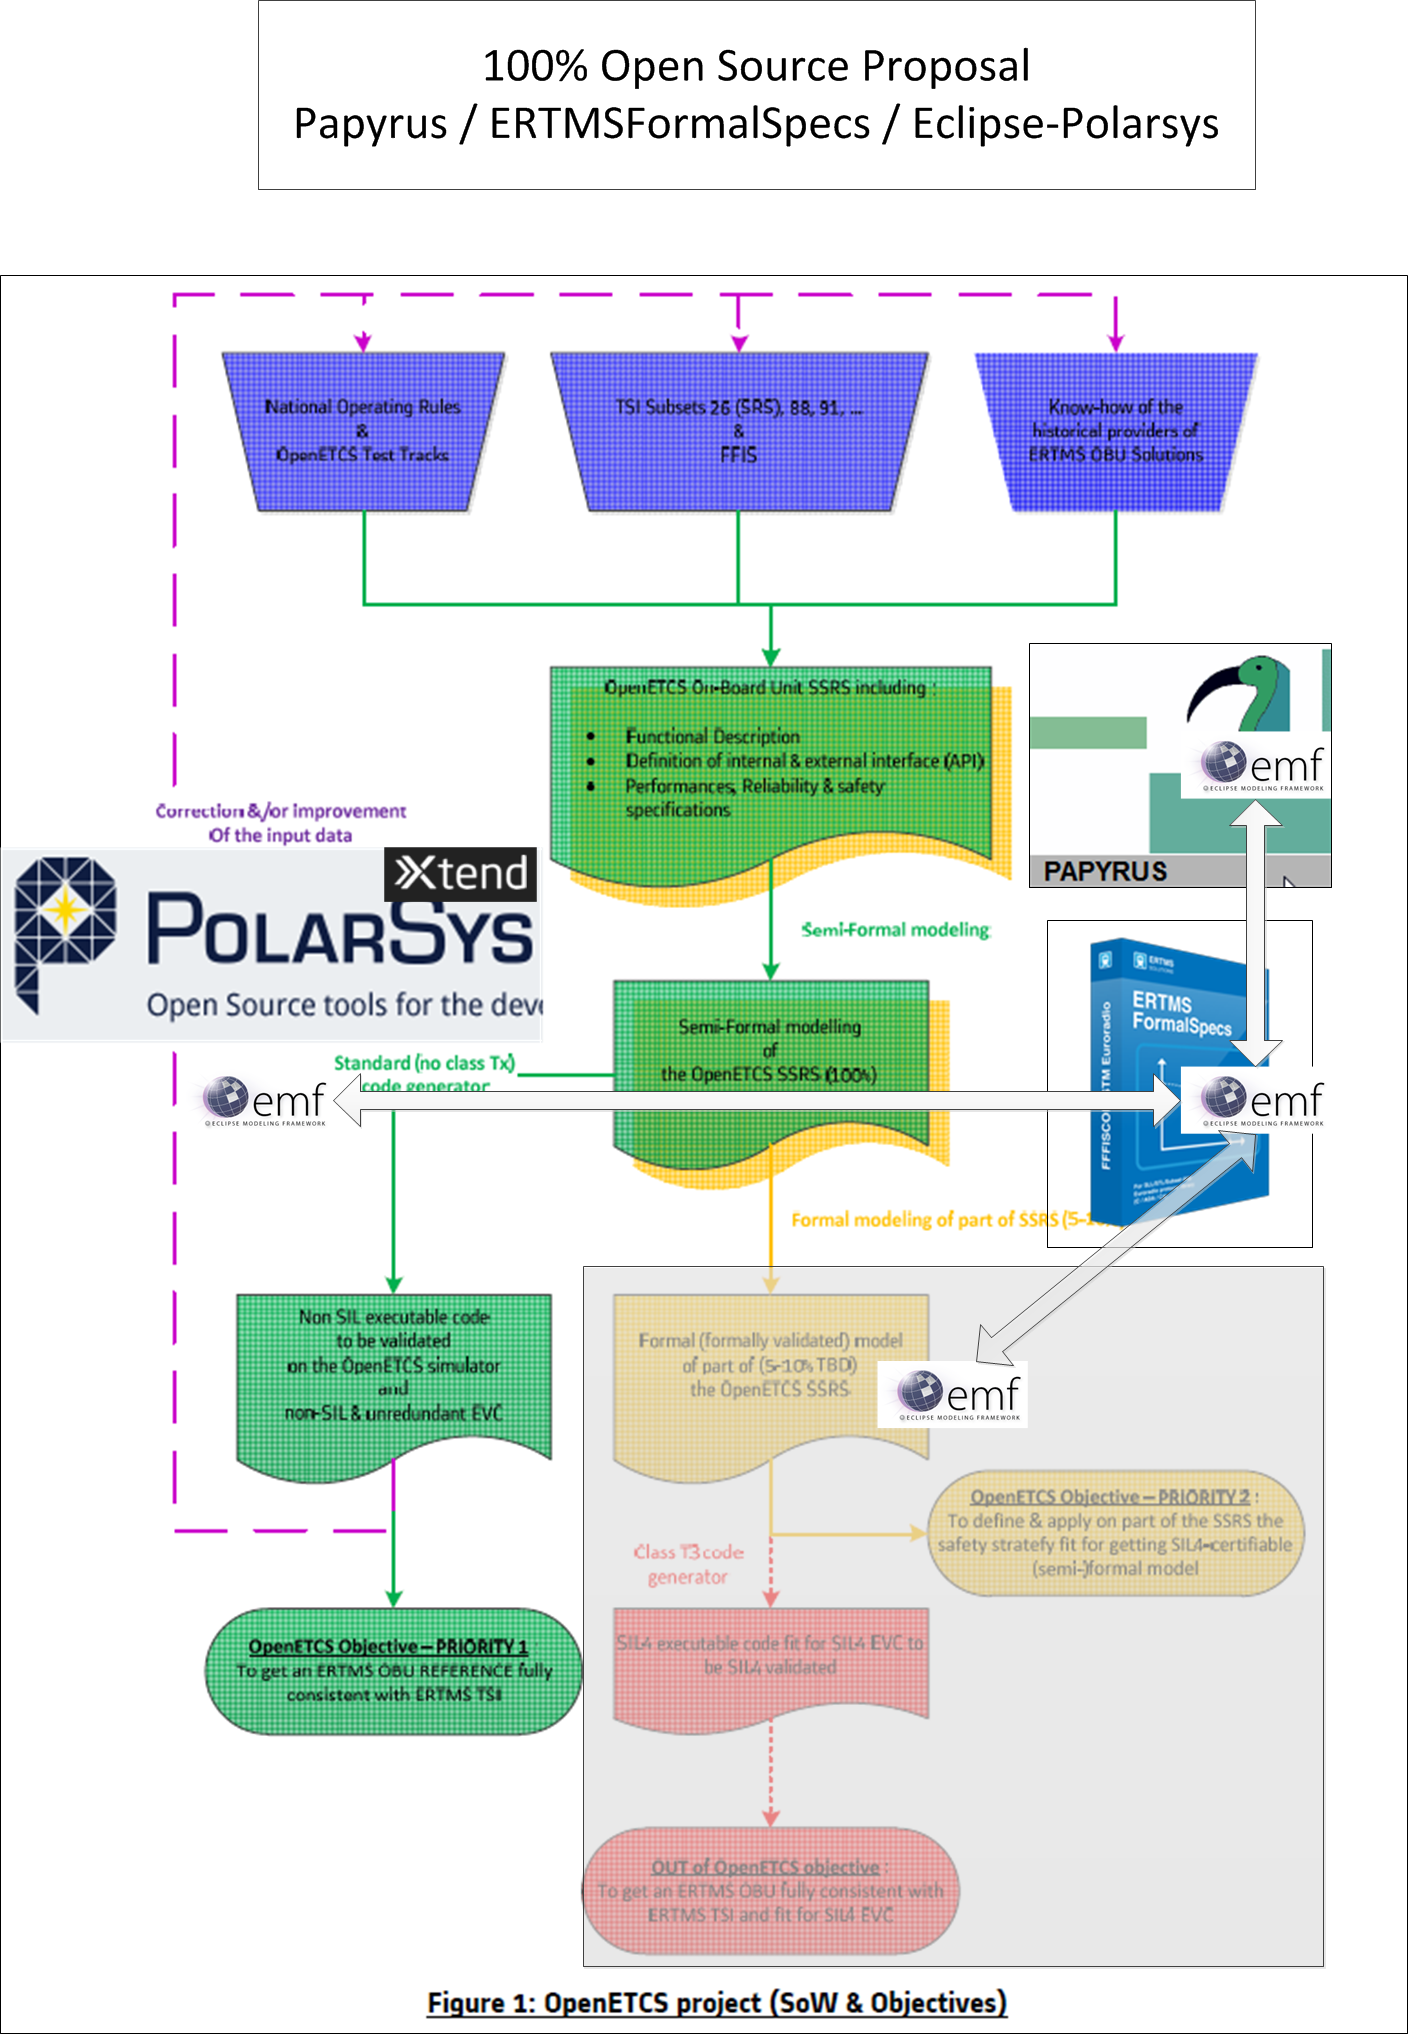
\includegraphics[width=1.10\textwidth]{images/ERTMSSolutionsAlt_1.png}
		\caption{SysML, ErtmsFormalSpec and Eclipse/Polarsys Proposal}
	\label{fig:ERTMSSolutionsAlt_1}
\end{figure}

\section{Description of the approach for OpenETCS design process}

The blue boxes of the overall design process are covered in the following manner:

SSRS box: Using Papyrus for modelling the high-level system design in SysML language. 

Sub-system semi-formal model box: Using ERTMSFormalSpecs to model the complete SSRS into a semi-formal model.

Software semi-formal model + architecture description box: Shall be done inside Eclipse/Polarsys tools for transforming a semi-formal model 
into software source code. The exact mix of Eclipse/Polarsys tools is to be decided by the participants of task T3.8. 

Target source code box: This box is covered by the source code generated by the Eclipse/Polarsys tools. This source code can then be compiled and executed on the demonstrator hardware. 

\section{Integration of the approach with SysML/Papyrus}

The proposed approach uses SysML/Papyrus as top-level component. Moreover, as SysML/Papyrus and ERTMSFormalSpecs both support an EMF-based interface, 
technical integration between both tools is not an issue.

As ERTMSFormalSpecs is already implementing 44\% of Subset-026, some questions are open:

- How can the SysML system-level model be connected with the ERTMSFormalSpecs semi-formal model? 
- Can a SysML system-level model be generated based on the existing 44\% of Subset-026, so that this SysML system-level model 
can then be improved, 

\section{Integration of the approach with Eclipse}

SysML/Papyrus is completely based on Eclipse.

ERTMSFormalSpecs supports today an EMF interface, enabling Eclipse-based tools to reuse the existing ERTMSFormalSpecs model. 

Eclipse/Polarsys tools are also based on Eclipse, raison no integration concerns.

\section{Benefits versus OpenETCS requirements}

The benefits of the SysML/Papyrus/ERTMSFormalSpecs/Eclipse/Polarsys proposal are the following:

\begin{itemize}
	\item As of today, already 44\% of Subset-026 requirements modelled. This proposal enables the OpenETCS project to start with a headstart, instead of nothing.
	\item ERTMSFormalSpecs is the only semi-formal candidate to have built-in braking curves modellings and visualization, verified with the ERA model
	\item ERTMSFormalSpecs has very strong support for traceability to the Subset-26, and to the Subset-076 for test cases
	\item ERTMSFormalSpecs has its domain-specific language, which is productive for this field, thanks to its expressivity, illustrated by the primitives
developed for braking curves and scalable, as is demonstrated by the large fraction of the Subset26 which has been represented so far
	\item Fully open-source (ERTMSFormalSpecs under EUPL license, others open source)
	\item ERTMSFormalSpecs model can be transformed automatically to SCADE model (confirmed by ESTEREL Technologies in Munich meeting), allowing to choose SCADE as a code generation backend in case Eclipse/Polarsys would not meet the project requirements
	\item The three elements of the toolchain (Papyrus, ERTMSFormalSpecs and Eclipse) boast an active community of users and are supported by open-source business cases
\end{itemize}

\section{Shortcommings versus OpenETCS requirements}

The shortcomings of the SysML/Papyrus/ERTMSFormalSpecs/Eclipse/Polarsys proposal are the following:

\begin{itemize}
	\item ERTMSFormalSpecs has a perfectible look and feel and lacks graphical rendering of the architecture. \emph{This shortcoming might be addressed with the integration of SysML as a language for the higher level architecture.}
	\item As of today, the code generation in Eclipse/Polarsys, transforming the ERTMSFormalSpecs in generated source code, is not yet available, and must be developed during task 3.8 of the project. \emph{This shortcoming can be mitigated by integrating the scade code generator as a itermediates solution.}
\end{itemize}

\section{On going work for openETCS project}

The following elements should be further developed during the OpenETCS project, to alleviate the shortcomings listed above:

\begin{enumerate}
  \item Develop conceptual and technical strategies to integrate SysML with ERTMSFormalSpecs model, going beyond the state-of-the-art. The state-of-the-art in integrating SysML models and industrial (semi-)formal languages being SCADESystem, in which only the module, interfaces and dataflows are connected to the lower-level model.
	\item Further develop ERTMSFormalSpecs model to cover 100\% of Subset-026, 100\% of Subset-076, and to fully test the model within ERTMSFormalSpecs. 
	\item Either implement a full eclipse-based version of the ERTMSFormalSpecs workbench for model development, traceability and testing, or improve the ERTMSFormalSpecs user interface to be fully productive for T3.5 and T3.6 tasks
	\item Develop code-generation strategies during T3.8 tasks
\end{enumerate}

Among theses tasks, Task 2 and 4 fit inside the WP3 existing tasks, and do not need additional skills than the ones present in the OpenETCS consortium as of today. Task 1 is also seriously represented in the consortium, in which a lot of SysML experience is present. 

Task 3 (porting the ERTMSFormalSpecs workbench to Eclipse) is a task that falls in the scope of WP7, and for which Eclipse development and integration skills are required.

\section{Conclusion and other comments}

As a conclusion, the SysML/Papyrus/ERTMSFormalSpecs/Eclipse/Polarsys proposal has as 3 key strengths 1/ to be fully available today, 2/ to already model 44\% of Subset-026, and 3/ to be fully open-source. 

Moreover, it proposes a realistic technical foundation to achieve the WP3 and projects top-priority objectives with the skills and resources available in the project.
